\documentclass[11pt]{article}
\usepackage[T1]{fontenc}
\usepackage[utf8]{inputenc}
\usepackage{lmodern,amsmath,amssymb,amsthm,mathtools,booktabs,array}
\usepackage[margin=1in]{geometry}
\usepackage{microtype,graphicx,enumitem}
\usepackage[colorlinks=true,allcolors=blue]{hyperref}
\newtheorem{theorem}{Theorem}[section]
\newtheorem{lemma}[theorem]{Lemma}
\newtheorem{proposition}[theorem]{Proposition}
\newtheorem{corollary}[theorem]{Corollary}
\theoremstyle{remark}\newtheorem{remark}[theorem]{Remark}
\newcommand{\norm}[1]{\left\lVert#1\right\rVert}
\newcommand{\abs}[1]{\left\lvert#1\right\rvert}
\newcommand{\fl}{\operatorname{fl}}
\newcommand{\tr}{\operatorname{tr}}
\newcommand{\spec}{\operatorname{spec}}
\newcommand{\R}{\mathbb R}
\newcommand{\C}{\mathbb C}
\newcommand{\unit}[1]{\mathcal U(#1)}
\DeclareMathOperator{\diag}{diag}
\title{Selected bidiagonal singular directions with fixed-format linear output work}
\author{Kaiwen Jin\\\small\texttt{yui.ui.siki@gmail.com}}
\date{October 15, 2026}
\begin{document}
\maketitle
\begin{abstract}
Computing a few singular vectors of a bidiagonal matrix requires control of
orthogonality as well as residuals when singular values cluster. We give a
rational-filter construction for any requested set of $k$ ordered singular
triplets of a real $n\times n$ upper bidiagonal matrix. For
$\epsilon=2^{-p}$, $16\le p\le53$ and $n\epsilon\le1/64$, its represented
unit directions satisfy both singular-vector residual bounds, ordered-value
accuracy and separate left and right orthogonality bounds with a universal
constant, independent of the input gaps. The work is $O(p^4nk)$ operations on
$O(p)$-bit numbers, or conservatively $O(p^6nk)$ bit operations. Thus the work
is linear in $nk$ after the format is fixed. The sufficient core precision is
220224 bits for a binary64 target; practical speed superiority is not claimed.
Count-separated spectral intervals, positive rational filters and joint
Schur-complement columns avoid a final vector reorthogonalization. A common
cut near zero permits recovery of left directions without a small-singular-value
assumption. The arithmetic model and the distinction between floating carriers
and exact unit directions are explicit. A research implementation supplies
separate proof and diagnostic configurations with optional exact checks of
finite outputs.
\end{abstract}

\section{Introduction}
The singular value decomposition of a dense matrix is commonly reduced to the
same problem for a bidiagonal matrix. If only a few singular triplets are
needed, the final bidiagonal stage should ideally require work proportional
to the number of returned entries. Small residuals alone do not ensure this:
vectors associated with a tight cluster can satisfy their individual equations
while being almost parallel. Selected triplets must satisfy both singular-vector
equations and must remain separately orthogonal on the left and on the right.

Gro{\ss}er and Lang~\cite{GL} studied an $O(n^2)$ bidiagonal SVD construction
using relatively robust representations. Their analysis identifies difficulties
with separately solving the two Gram eigenproblems, and with tiny clusters
in the Jordan--Wielandt formulation. Marques, Demmel and
Vasconcelos~\cite{MDV} developed selected bidiagonal SVD computation through
an associated symmetric tridiagonal eigenproblem. Their report discusses
the care required in extracting singular vectors and the limitations of
available clustered-eigenvector computations. These are different issues from
obtaining a small individual eigenpair residual.

Problem 3.8 of Amsel et al.~\cite{open} asks for $O(nk)$ bidiagonal singular-vector
work together with residual and orthogonality guarantees. We make the
arithmetic and output conventions explicit. Our target additionally requires
accuracy at each requested ordered singular value and both residual equations.
The construction below has a universal error constant for these simultaneous
requirements. Its $O(nk)$ statement concerns a fixed format: the precision
dependence is $O(p^4nk)$ multiprecision operations. We represent an exact unit
direction by a nonzero floating carrier $x$ with meaning
$x/\sqrt{x^Tx}$; the raw arrays satisfy a separate perturbation bound.

Informally, for any stored real upper bidiagonal input and any distinct
requested ranks, we obtain nonnegative singular estimates and unit directions
with value and residual errors at most $128n\epsilon\norm{B}_2$ and pairwise
inner products at most $128n\epsilon$. No separation between neighboring input
singular values is assumed. The construction uses correctly rounded real
operations with protected exact index and scaling arithmetic, excluding
overflow and underflow. Its very conservative precision makes it a complexity
construction rather than a proposed replacement for standard SVD software.

The first difficulty is to make the requested vectors joint rather than
independent approximations. Protected inertia counts produce disjoint spectral
intervals whose endpoints lie in gaps chosen by the algorithm. A positive
rational approximation to each interval projector permits successive
Schur-complement columns. A trace estimate chooses their coordinates while
controlling a single orthogonal comparison family. Semiseparable resolvent
representations make each coordinate scan linear in the matrix order.

The second difficulty is finite arithmetic in repeated shortening and recovery
near zero. We compare the supplied generators with one nearby filter and bound
scan errors over an entire segment, avoiding a product of local stability
constants over the matrix order. For recovery, one common cut of the squared
spectrum divides the small-value and positive branches. The near-kernel bound
on a left direction cancels the apparent reciprocal small-value loss in its
inner product with a positive left direction.

Section~\ref{sec:model} gives the model and main result.
Sections~\ref{sec:counts}--\ref{sec:round} construct and analyze the joint
tridiagonal procedure. Section~\ref{sec:recovery} proves the bidiagonal
recovery and rounding bounds, and Section~\ref{sec:software} describes the
implementation and finite validation. Vector norms are Euclidean and matrix
norms are spectral unless stated otherwise. A superscript $T$ is an ordinary
transpose, including in complex symmetric formulas; $*$ denotes an adjoint.

\section{Task, arithmetic and output}\label{sec:model}
Let $B\in\R^{n\times n}$ have diagonal $d_1,\ldots,d_n$ and superdiagonal
$e_1,\ldots,e_{n-1}$. The input entries are the stored real floating numbers,
not unknown numbers before input rounding. Write its singular values as
$\sigma_1\ge\cdots\ge\sigma_n\ge0$. The requested indices
$j_1,\ldots,j_k$ are distinct elements of $\{1,\ldots,n\}$, with $1\le k\le n$.

Fix $p\in\{16,\ldots,53\}$ and put $\epsilon=2^{-p}$. The output carriers
and singular estimates use binary64 storage; $p<53$ requests a looser target
for that same stored input. Basic real addition, subtraction, multiplication,
division and square root at each specified internal precision are rounded to
nearest. Complex arithmetic is expanded into these real operations. Protected
integer indices, count-grid operations and power-of-two exponents are exact.
Overflow and underflow are excluded. Input exponent costs belong to the fixed
input format. The mathematical result is under this arithmetic model, rather
than a formal verification of a language, compiler or library.

For each nonzero real carrier $x$, define
\begin{equation}\label{eq:unit}
  \unit{x}=\frac{x}{\sqrt{x^Tx}}.
\end{equation}
An output $(\widehat\sigma,x,y)$ represents the exact mathematical triplet
$(\widehat\sigma,\unit{x},\unit{y})$. Equation~\eqref{eq:unit} specifies
the direction represented by a finite array; it is not an assertion that an
array has exactly unit floating norm. Constructing, copying and approximately
materializing the directions is charged. An explicitly requested exact
squared norm is a separately paid rational sum; no exact irrational floating
primitive is assumed.

\begin{theorem}\label{thm:main}
Suppose $n\epsilon\le1/64$ under the preceding model. For every such $B$ and
every set of $k$ distinct requested indices, the algorithm below returns
nonnegative binary64 estimates $\widehat\sigma_i$ and nonzero binary64
carriers $x_i,y_i$. With $\widehat u_i=\unit{x_i}$ and
$\widehat v_i=\unit{y_i}$,
\begin{align}
 \abs{\widehat\sigma_i-\sigma_{j_i}(B)}&\le128n\epsilon\norm B,\label{eq:value}\\
 \norm{B\widehat v_i-\widehat\sigma_i\widehat u_i},\quad
 \norm{B^T\widehat u_i-\widehat\sigma_i\widehat v_i}
   &\le128n\epsilon\norm B,\label{eq:res}\\
 \abs{\widehat u_i^T\widehat u_j},\quad
 \abs{\widehat v_i^T\widehat v_j}&\le128n\epsilon\quad(i\ne j).\label{eq:orth}
\end{align}
Also $\abs{x_i^Tx_i-1},\abs{y_i^Ty_i-1}\le8\epsilon$.
The constant is independent of all singular-value gaps and clusters.
The complete production work is $O(p^4nk)$ operations on $O(p)$-bit numbers;
elementary multiprecision arithmetic gives the conservative bit bound
$O(p^6nk)$. The sufficient kernel precision is $67584+2880p$ bits, including
220224 bits when $p=53$.
\end{theorem}

Here $n$ is the matrix order, $k$ the number of requested ranks and $\epsilon$
the target error scale. Repeated values permit any orthonormal directions in
their subspace. Signed, reducible and singular matrices are included. Fixing
the format makes the displayed operation bound $O(nk)$ in $n,k$; the theorem
does not give a precision-uniform $O(nk)$ bound.

\subsection{The bidiagonal procedure}
For $B\ne0$, let $\rho=\max(\abs{d_i},\abs{e_i})$ and choose a power of two
$s$ with $2\rho\le s\le4\rho$. Set
\begin{equation}\label{eq:scales}
 A=B/s,\qquad G_R=A^TA,\quad G_L=AA^T,\qquad
 \Delta=n\epsilon,\quad \xi=2^{-20}n\epsilon^3,\quad q=3p+32.
\end{equation}
The row and column sums of a bidiagonal matrix give
$1/4\le\norm A\le1$ and $s\le4\norm B$. Both raw Grams are tridiagonal
and satisfy $0\le G_R,G_L\le I$. Their local products are formed from the
stored input at the specified precision, not from a binary64 rounded Gram.
They have the same ordered eigenvalues with multiplicity.

The tridiagonal procedure analyzed below returns jointly controlled directions
and centers for any requested ranks of $G$. For accuracy $\eta=2^{-q}$ its
value, residual and pairwise inner-product errors are at most $512n\eta$.
Call this procedure $\operatorname{JointGram}(G,J,q)$.

\begin{center}
\fbox{\begin{minipage}{.94\linewidth}
\textbf{Algorithm 1: selected bidiagonal singular directions.}
Input: stored $d\in\R^n$, $e\in\R^{n-1}$, distinct ranks $J=(j_i)_{i=1}^k$,
and $p$ with $n2^{-p}\le1/64$.
\begin{enumerate}[leftmargin=*,nosep]
\item If $B=0$, return the requested distinct coordinate vectors on both sides
and zero values. Otherwise form~\eqref{eq:scales}.
\item Use protected counts of $G_R$ to find a common cut
$\theta\in[\Delta^2,2\Delta^2]$ with clearance
$\gamma>\Delta^2/(64n)$. Let $m_0$ be the exact number below the cut.
\item Call $\operatorname{JointGram}(G_R,J,q)$ once for all requested right
directions $v_i$ and centers $\alpha_i$.
\item Call $\operatorname{JointGram}(G_L,J_0,q)$ once, only for requested
indices $J_0=\{j_i:j_i>n-m_0\}$, giving $w_i,\beta_i$.
\item For $j_i\notin J_0$, compute $t_i=\norm{Av_i}$,
$u_i=Av_i/t_i$ and $\widetilde\sigma_i=st_i$. For $j_i\in J_0$,
set $u_i=w_i$ and $\widetilde\sigma_i=0$.
\item Round values and carriers only after this recovery; return their unit
representations~\eqref{eq:unit} in requested order.
\end{enumerate}
Output: $k$ nonnegative values and $k$ left/right carriers. Optional exact
instance verification is outside this production algorithm.
\end{minipage}}
\end{center}

The safe cut costs $O(n\log(n+1))$ work. Packet placement and localization cost
$O(nk[q+\log(n+1)])$. With rational rank $r=O(q^2)$, coefficient construction
costs $O(r)$ per packet, supply costs $O(nr)$, each selected scan $O(nr^2)$
and each selected solve/matvec $O(nr)$. There are at most $k+k_0\le2k$
requested Gram columns. Since $\log n\le p$, these costs, recovery and output
give $O(p^4nk)$. Storage is $O(nk+nr+r^2)$ high-precision words, with
output, controller and one packet workspace counted. No full spectrum,
$n\times n$ projector, entire null space, or final $k$-vector
reorthogonalization is computed.

\section{Protected counts and rational interval filters}\label{sec:counts}
We first separate spectral intervals without a promise on the input gaps.
The spectral theorem for real symmetric matrices~\cite[Theorem 7.29]{Axler}
gives ordered eigenvalues and orthogonal projectors. Its min--max formula
implies $\abs{\lambda_j(T)-\lambda_j(H)}\le\norm{T-H}$: each unit Rayleigh
quotient changes by at most this norm, and one takes the same minima and
maxima. Invertible congruence preserves inertia because it preserves the
maximum dimension of a strictly negative quadratic subspace. These facts
justify the protected counts that follow.

\subsection{Counts and rank localization}
Put $Q=2^{12q}$, $\tau=\eta^4$ and $\beta=\tau+4/Q$. Round each
tridiagonal entry to the $1/Q$ grid. At a grid shift $z$ evaluate the scalar
$LDL^T$ recurrence, rounding each quotient to this grid. Replace a pivot of
magnitude below $\tau$ by the same-signed $\tau$, assigning a zero pivot
the negative sign. Count the negative pivots.

These pivots are exact factors of a nearby tridiagonal: the quotient rounding
and pivot replacement alter a diagonal entry by at most $\tau+1/(2Q)$.
Entry rounding contributes norm error below $2/Q$. Thus, if
$N(z)=\#\{\lambda<z\}$ and $c(z)$ is the computed count,
\begin{equation}\label{eq:soft}
 N(z-\beta)\le c(z)\le N(z+\beta).
\end{equation}
Every division is defined. Pivot sizes and quotient numerators have $O(q)$
bits, apart from the fixed input exponent cost. A count costs $O(n)$
operations. Although adjacent counts need not be monotone,~\eqref{eq:soft}
gives $c(x)\le c(y)$ whenever $y-x\ge2\beta$.

For $H=2I+G$, $0\le G\le I$, counts at the endpoints certify the interval
$[1/2,4)$. To locate descending rank $j$ (one based), target ascending rank
$n+1-j$. At a midpoint $z$, update the lower endpoint to
$\max(\mathrm{lo},z-\beta)$ if $c(z)<n+1-j$; otherwise update the upper
endpoint to $\min(\mathrm{hi},z+\beta)$. The exact eigenvalue remains in the
closed bracket. Its width obeys $w_{\mathrm{new}}\le w/2+\beta+1/(2Q)$;
after $2q+10$ steps it is at most $\eta^2/64$.

For the integer search define $c_g(Z)=c(Z/Q)$ and $\beta_g=Q\beta$.
The integer coordinate $Z$ represents the spectral coordinate $Z/Q$.
\begin{lemma}\label{lem:gap}
Suppose the integer interval $[L_g,R_g]$ has safe population upper bound
$r_0=c_g(R_g+\beta_g)-c_g(L_g-\beta_g)$, and an integer
$h_g\ge\max(1,4\beta_g)$ satisfies $R_g-L_g\ge(12r_0+4)h_g$.
A deterministic search finds an integer center at distance at least $h_g$
from the rescaled spectrum and its exact count in $O(\log(n+1))$ count calls.
\end{lemma}
\begin{proof}
At the integer midpoint $x_g$, equality of $c_g(x_g-h_g-\beta_g)$ and
$c_g(x_g+h_g+\beta_g)$ certifies the required interval. If they differ,
discard $[x_g-2h_g,x_g+2h_g]$. The safe population bounds of the two remaining
sides have sum at most $r_0-1$, by the separated-query ordering above.
Choose the side with smaller population. Its length is at least
$(R_g-L_g-1)/2-2h_g$, sufficient for the same length condition with the new
population. Each failure halves the population; population zero succeeds
immediately. The midpoint rounding is absorbed by $h_g\ge1$.
\end{proof}
Each application below uses $L_g=QL$, $R_g=QR$ and $h_g=Qh$; the chosen
dyadics make these integers. Dividing the returned center and clearance by
$Q$ restores spectral units, with physical clearance $h$.

Take the largest dyadic $W\le n\eta/4$, so $W>n\eta/8$. At each anchor
$aW$ choose a boundary in $[aW-W/4,aW+W/4]$ by Lemma~\ref{lem:gap},
with the largest dyadic $h\le W/[2(12n+4)]$. Here $h>\eta/512$
exceeds both $1/Q$ and $4\beta$, and the length $W/2$ meets the
rescaled lemma's length condition. Cache this deterministic choice
by its integer anchor. Consecutive boundaries are between $W/2$ and $3W/2$
apart. A localized requested rank belongs, by the exact boundary counts, to
one of three neighboring cells. At most three boundaries per request suffice.
We call a cell a spectral packet. Distinct packets are disjoint, their
halfwidths are at most $3n\eta/16$, and their endpoint clearance satisfies
$h>\eta/512$. This proves the setup cost stated after Algorithm 1.

Applying the same search to $G_R$ on $[\Delta^2,2\Delta^2]$ with the largest
dyadic $h\le\Delta^2/(32n)$ gives
\begin{equation}\label{eq:cut}
 \Delta^2\le\theta\le2\Delta^2,\qquad
 \operatorname{dist}(\theta,\spec G_R)\ge\gamma=h>\Delta^2/(64n).
\end{equation}
For $q=3p+32$, the length condition holds and
$h>\Delta^2/(64n)\ge\epsilon^2/64>\max(1/Q,4\beta)$,
so $Qh\ge\max(1,4Q\beta)$. Both Grams share
this cut and count. The gap in~\eqref{eq:cut} is chosen by the algorithm,
not imposed on the input singular values.

\subsection{A positive rational approximation}
For a packet $(l,u)$ of $H$, let $\mu=(l+u)/2$, $a_0=(u-l)/2$,
$a=a_0-h/2$ and initially $g=a_0+h/2$. The two exterior neighboring ranks
may be localized to increase $g$, while retaining $0<a<g\le8$. Target
eigenvalues satisfy $\abs{\lambda-\mu}\le a$ and exterior eigenvalues
satisfy $\abs{\lambda-\mu}\ge g$. Set
\[
 \ell=\frac{g-a}{g+a}\ge\frac1{512n},\qquad
 y(x)=\frac{(x-\mu)^2-ag}{(x-\mu)^2+ag}.
\]
The target has $y\le-\ell$, and the exterior has $y\ge\ell$;
$\sqrt{ag}\ell\ge h/4$. A whole-space packet needs only coordinate
directions and requires no rational filter.

Starting with $r_0(y)=y$ and $\ell_0=\ell$, define
\begin{equation}\label{eq:sign}
 \alpha_t=\ell_t^{-1/2},\quad
 r_{t+1}(y)=\frac{2\alpha_t r_t(y)}{1+\alpha_t^2r_t(y)^2},\quad
 \ell_{t+1}=\frac{2\sqrt{\ell_t}}{1+\ell_t}.
\end{equation}
For $\ell\le\abs y\le1$,
$\ell_t\le\operatorname{sign}(y)r_t(y)\le1$. Indeed the scalar map has
maximum 1 at $\sqrt{\ell_t}$ and equal endpoint minima $\ell_{t+1}$.
After $\lceil\log_2(q+3)\rceil$ steps $\ell_t\ge1/2$. Subsequently,
$z_t=(1-\ell_t)/(1+\ell_t)$ satisfies $z_{t+1}\le z_t^2$ and $z_t\le1/3$.

Let $\delta=2^{-20}\eta^6$ and
\[
 J_{\max}=\lceil\log_2(q+3)\rceil+
            \lceil\log_2(6q+27)\rceil\le19.
\]
The iteration count is selected without a precision retry. With
$Q_s=2^{768+16q}$ and $L_0=\lfloor Q_s\ell\rfloor$, use
\begin{equation}\label{eq:down}
 L_{t+1}=\left\lfloor
 \frac{2\lfloor\sqrt{L_tQ_s}\rfloor Q_s}{Q_s+L_t}
 \right\rfloor
\end{equation}
until $L_t/Q_s\ge1-\delta/16$. Each downward local defect is below $3/Q_s$.
The map in~\eqref{eq:sign} contracts logarithmic input errors by at most
$1/2$. Its accumulated lower-bound defect is at most
$16(J_{\max}+1)/(Q_s\ell_{\min})<\delta/64$, where
$\ell_{\min}=1/(512n)$. The ideal endpoint error is below $\delta/64$
by $J_{\max}$, so the stated stopping threshold is attained by then.
For the exact packet projector $\Pi$, putting $\vartheta=\delta/4$ gives
\begin{equation}\label{eq:filter}
 F_0=\frac{(I-r_J(y(H)))/2+\vartheta I}{1+2\vartheta},
 \qquad \delta I/8\le F_0\le I,\quad \norm{F_0-\Pi}\le\delta.
\end{equation}

\subsection{Coefficients without subtractive residue formulas}
Write $\psi_\alpha(x)=2\alpha x/(1+\alpha^2x^2)$. For $b,W>0$ and
$t=\sqrt{1+b^2}$,
\begin{align}\label{eq:transport}
 \frac{W\psi_\alpha(x)}{\psi_\alpha(x)^2+b^2}
 &=\frac{W_-x}{x^2+b_-^2}+\frac{W_+x}{x^2+b_+^2},\\[-4pt]
 b_-&=\frac b{\alpha(1+t)},& b_+&=\frac{1+t}{\alpha b},\nonumber\\
 W_-&=\frac W{\alpha t(1+t)},&W_+&=\frac{W(1+t)}{\alpha t b^2}.\nonumber
\end{align}
Common denominators verify the identity. Starting with
$(b,W)=(1/\alpha_{J-1},2/\alpha_{J-1})$ and transporting backwards gives
the partial fractions of $r_J$. All magnitude operations are positive; no
subtraction such as $1-\alpha^2b^2$ is evaluated. The full conjugate rank is
$r=2^{J+1}=O(q^2)$ and $r\le2^{20}$; construction costs $O(r)$.

For completeness, positive addition is nonexpansive in the maximum
logarithmic input error and a rounded real operation adds at most $2u$.
The scale recurrence has logarithmic derivative at most $1/2$, giving scale
and $\alpha$ errors at most $12u$ and $10u$. The inverse-branch logarithmic
derivatives in $b$ are $\pm1/t$, and those for $W$ have magnitude at most 3.
After $v$ levels, $e_b\le(12+20v)u$ and
$e_W(v+1)\le e_W(v)+3e_b(v)+30u$. Therefore
\begin{equation}\label{eq:coeflog}
 \max\{\abs{\log(\widehat b/b)},\abs{\log(\widehat W/W)}\}
 \le128(J+1)^2u.
\end{equation}
The initial packet data are dyadics imported exactly before the controlled
division. The logarithmic derivative bounds hold throughout the positive
domain, so this is a finite perturbation estimate.

Each $b$ gives poles
\[
 z=\mu\pm\frac{\sqrt{ag}}{\sqrt{1+b^2}}
       +i\frac{\sqrt{ag}b}{\sqrt{1+b^2}}
\]
and their conjugates. The corresponding weights are
$-W\sqrt{ag}(1+ib)/[4(1+2\vartheta)(1+b^2)^{3/2}]$ and the negative
conjugate, paired with those poles. Real and imaginary components are formed
separately; cancellation in the real center is bounded absolutely.
Reverse transport gives $\min(b,1/b)\ge\ell/3^J$: each reverse level loses
at most $3\alpha$, while the product of the inverse scales with the starting
$\sqrt{\ell_{J-1}}$ is at least $\ell$. Also
$r_J(1)=\sum W/(1+b^2)\le1$, so the ideal absolute weight mass is at most
$\sqrt{ag}$. The ideal pole clearance is greater than $2^{-44}\eta$;
rounded poles have clearance at least $2^{-48}\eta$. Conservatively the
stored weight mass is at most 16, the constant magnitude at most 2 and
$\max(1,\norm H+\abs z)\le32$.

At $b_{\rm coef}=1024+16q$ bits, resolvent identities and
\eqref{eq:coeflog} bound the common coefficient-operator error by
$2^{136}u_{\rm coef}\eta^{-2}$. The two inverse-clearance factors account
for a pole perturbation. Rounding the raw tridiagonal contributes at most
$2^{104}u_s\eta^{-2}$ with $u_s=2^{-(768+16q)}$.
The wider core imports the stored dyadic coefficients exactly.

\section{Joint columns from a positive structured filter}\label{sec:columns}
This section describes the exact column selection and structured operations
whose finite arithmetic is treated in Section~\ref{sec:round}.
Let $0<F\le I$ approximate a packet projector of population $s_0$.
For a selected coordinate set $I_t$, put
\[
 C_t=F[I_t,I_t],\quad
 R_t=F-F[:,I_t]C_t^{-1}F[I_t,:],\quad f_t=\tr(C_t^{-1}),\quad f_0=0.
\]
An unselected coordinate $j$ has shorted diagonal $d_j=(R_t)_{jj}$ and
squared interpolation norm $h_j=\norm{C_t^{-1}F[I_t,j]}^2$.
Choose a coordinate whose score $(1+h_j)/d_j$ is within twice the minimum,
and normalize the column $R_te_j$. Repeat only for the number of requested
directions in the packet.

\begin{lemma}\label{lem:selection}
If $\tr F\ge s_0-1/2$ and $t\le s_0$, twice-minimum selection satisfies
$f_t\le4n^3$. If $\norm{F-\Pi}\le\delta_{\rm eff}$ with the smallness
conditions below, the selected unit columns are close to a single orthogonal
family in $\operatorname{range}\Pi$.
\end{lemma}
\begin{proof}
Block inversion gives $f_{t+1}=f_t+\mathrm{score}_{\rm chosen}$.
From $F^2\le F$, the sum of the score numerators is at most $n-2t+f_t$,
and the sum of their denominators is at least $q_0-t$, with $q_0=s_0-1/2$.
Thus
\[
 f_{t+1}\le f_t+\frac{2(n+f_t)}{q_0-t},\qquad
 f_t\le n\left[
 \frac{(q_0+1)(q_0+2)}{(q_0-t+1)(q_0-t+2)}-1\right]\le4n^3.
\]
The formula follows by multiplying the recurrence for $n+f_t$.
Every selected shorted diagonal is at least $1/(4n^3)$.

Set $H_t=\max(1,f_t)$. The corresponding selected block of $\Pi$ has
minimum eigenvalue at least $1/H_t-\delta_{\rm eff}$. Partition
$\Pi=\left[\begin{smallmatrix}C&D^T\\D&E\end{smallmatrix}\right]$.
Since $\Pi^2=\Pi$, $D^TD=C-C^2$, and
$X=[-C^{-1}D^T;I]$ satisfies $\norm X^2\le1/\lambda_{\min}(C)$.
Block elimination and a resolvent expansion of the selected inverse bound
the shorting perturbation by
\[
 \frac{\delta_{\rm eff}H_t}{1-2\delta_{\rm eff}H_t}
 \le2\delta_{\rm eff}H_t.
\]
For $\delta=2^{-20}\eta^6$ and $\delta_{\rm eff}\le2\delta$, the chosen
ideal remaining projector diagonal is at least $1/(8n^3)$. The normalization
inequality
$\norm{a/\norm a-b/\norm b}\le2\norm{a-b}/\norm b$ gives unit-column
distance at most $128\delta n^{9/2}\le n\eta/4096$.
Successive shortenings of the same projector produce orthogonal ideal
columns. Projectors of disjoint packets are orthogonal as well.
\end{proof}

\subsection{Semiseparable recurrences}
A tridiagonal resolvent has a semiseparable representation. After combining
the conjugate poles, store scalars $a_i$, column generators
$u_i,v_i\in\C^r$ and diagonal propagators $P_i\in\C^{r\times r}$ such that
\begin{equation}\label{eq:ss}
 F_{ij}=u_i^TP_i\cdots P_{j+1}v_j\quad(i>j),\qquad F_{ji}=F_{ij}.
\end{equation}
We will ensure $\norm{P_i}\le1$. All contractions here are bilinear
transposes, as required by a complex symmetric resolvent; pairing yields a
real symmetric $F$.

For a fixed selected set, add $z$ to all selected diagonal entries at once.
A prime denotes the derivative at $z=0$. The forward state $S\in\C^{r\times r}$
and $S'$ start at zero before the first site. At site $i$, first
replace $S$ by $P_iSP_i^T$ (omitting the initial propagation); the scalar
$a_i(z)=a_i+z\mathbf 1_{i\in I_t}$ is the shifted diagonal. The resulting state gives
\begin{equation}\label{eq:forward}
 d_i=a_i-u_i^TSu_i,\quad b_i=v_i-Su_i,\quad
 w_i=b_i/d_i,\quad S_{\rm new}=S+b_ib_i^T/d_i
\end{equation}
at a selected site; an unselected site does not update $S$.
Differentiate all these expressions to propagate $S'$.
The backward state $\mathsf B\in\C^{r\times r}$ and its derivative
start at zero beyond the last site and satisfy
\begin{equation}\label{eq:backward}
 \mathsf B_{\rm new}=(I-u_iw_i^T)\mathsf B(I-w_iu_i^T)+u_iu_i^T/d_i
\end{equation}
at a selected site, followed by the appropriate $P_i$ propagation.
Differentiate this expression for $\mathsf B'$. At an unselected site,
\[
 d_j^{\rm short}=d_j-b_j^T\mathsf B b_j,\qquad
 h_j=d_j'-2(b_j')^T\mathsf B b_j-b_j^T\mathsf B'b_j.
\]
These give all scores with $O(nr^2)$ work and $O(nr+r^2)$ storage.
The reverse derivative involves blocks of the inverse square of the whole
selected matrix, rather than squares of isolated inverse blocks.

The stored $d_i,w_i$ also give streaming forward and reverse triangular solves
for $C_t^{-1}F[I_t,j]$. Multiplication by $F$ uses two length-$r$ states:
one forward state accumulates the strictly lower triangle of~\eqref{eq:ss}
and one reverse state the strictly upper triangle. Both the solve and matvec
cost $O(nr)$. They produce $R_te_j$ without storing a dense $F$ or $R_t$.

\section{Finite arithmetic and the inner Gram guarantee}\label{sec:round}
We now justify that the actual coefficients, generator supply, score scans
and column computations satisfy the hypotheses just used. All bounds are
conservative. The inner range needed for Algorithm 1 is $80\le q\le191$;
the estimates below hold for $16\le q\le244$ when $n\eta\le1/64$.

\subsection{One common nearby filter}
Within this subsection write $d_i=T_{ii}$ and $e_i=T_{i,i+1}$ for
the entries of the rounded real symmetric tridiagonal $T$. Write its
stored rational filter as
\[ F_{\rm coef}=fI+\sum_{\nu=1}^r\omega_\nu(T-z_\nu I)^{-1}. \]
Here $f$ is the real constant, $z_\nu$ the nonreal poles and
$\omega_\nu$ their weights, paired by conjugation as constructed above.
For a single pole $z$ and weight $\omega$, let
$\gamma_z=\abs{\Im z}$ and $L_z\ge\max(1,\norm T+\abs z)$.
The computed left and right pivots are
\begin{equation}\label{eq:pivots}
 p_i=d_i-z-e_{i-1}^2/p_{i-1},\qquad
 q_i=d_i-z-e_i^2/q_{i+1},
\end{equation}
with endpoint terms omitted. The inverse diagonal is computed from the
two-sided twist, $g_i=1/(p_i-e_i^2/q_{i+1})$.
Complex multiplication and division, expanded into real primitives, have
normwise errors at most $16u\abs{xy}$ and $16u\abs{x/y}$ for
$u\le1/8192$; complex addition/subtraction has error at most
$2u(\abs x+\abs y)$. The positive division denominator is
$(\Re y)^2+(\Im y)^2$. No relative componentwise cancellation bound is used.

For an upper-half-plane pole the pivot imaginary recurrences subtract
nonnegative terms from $-\gamma_z$. Their magnitudes stay at least
$\gamma_z/2$. Each local pivot defect is at most
$d_0=128uL_z^2/\gamma_z$. Thus all left pivots are exact pivots of
$A_L=T-zI+\diag(e_L)$ with $\abs{e_L}\le d_0$, and similarly on the right.
If $u\le\gamma_z^2/(8192L_z^2)$, then
\[
 -\Im A_L\ge\gamma_zI/2,\quad \norm{A_L}\le2L_z,\quad
 \norm{A_L^{-1}}\le2/\gamma_z.
\]
The identity
$\Im(A_L^{-1})=-A_L^{-*}(\Im A_L)A_L^{-1}$ gives
$\abs{(A_L^{-1})_{ii}}\ge\gamma_z/(8L_z^2)$. Consequently every
contiguous product of left propagations is at most
$P_0=16L_z^2/\gamma_z^2$. Comparing the mixed left/right twist matrix
first with $A_L$ and then with $T-zI$ gives
\begin{equation}\label{eq:twist}
 \abs{\widehat g_i-(A_L^{-1})_{ii}}
 \le4096uL_z^2/\gamma_z^3,\qquad \abs{\widehat g_i}\le3/\gamma_z.
\end{equation}
Zero offdiagonal entries give zero propagation and require no division by an
offdiagonal entry. Conjugate channels remain exact conjugates under symmetric
real rounding.

For raw propagation $\widehat\phi_{i+1}=\fl(-e_i/\widehat p_i)$,
form positive scales $\widehat s_1=1$ and
\[
 \widehat s_i=\fl\left(
  \sqrt{\fl(1+\fl((\fl(\abs{\widehat\phi_i}\widehat s_{i-1}))^2))}
       (1+128u)\right).
\]
Store $\widehat U_i=\fl(\fl(\omega\widehat g_i)\widehat s_i)$,
$\widehat V_i=\fl(1/\widehat s_i)$ and
$\widehat P_i=\fl(\widehat\phi_i\fl(\widehat s_{i-1}/\widehat s_i))$.
The scales cancel algebraically in represented offdiagonal products. Per-edge
relative errors are at most $128u$, and complete product errors are at most
$1024nu$ for $u\le1/(8192n)$. The outward factor dominates the scale and
ratio errors below $16u$, so $\abs{\widehat P_i}\le1$.
Expanding the positive scale recurrence using $P_0$ gives
\[
 1\le\widehat s_i\le4\sqrt n P_0,\qquad
 \abs{\widehat U_i}\le512\abs\omega\sqrt nL_z^2/\gamma_z^3.
\]
The diagonal is accumulated separately and is not identified with an exact
sum of the stored scaled generators.

For $r$ paired channels and $u\le1/(1024r)$, the actually represented
real symmetric filter satisfies
\begin{equation}\label{eq:supply}
 \norm{F_{\rm sup}-F_{\rm coef}}\le uC_{\rm sup},\qquad
 C_{\rm sup}=2^{20}n^2\sum_z\frac{\abs{\omega_z}L_z^4}{\gamma_z^5}
       +2^{10}r\left(\abs f+\sum_z\frac{\abs{\omega_z}}{\gamma_z}\right).
\end{equation}
Indeed an offdiagonal entry differs from $\omega(A_L^{-1})_{ij}$ by at most
\[
 \abs\omega P_0\left(4096uL_z^2/\gamma_z^3+
                          (3/\gamma_z)1024nu\right)
 \le2^{17}\abs\omega nuL_z^4/\gamma_z^5.
\]
Resolvent comparison with $T-zI$ and a maximum-row-sum bound give the first
term in~\eqref{eq:supply}. The rounded diagonal accumulation adds at most
$2^8ru(\abs f+\sum\abs\omega/\gamma_z)$, covered by the second term.
Every channel is compared with the same original $T$. Together with the
coefficient and input errors this gives one filter for every selected column.

\subsection{Segment bounds for the state scans}
Let an actually supplied $F$ satisfy $cI\le F\le I$ and~\eqref{eq:ss}
with contractive $P_i$. Let $U,V$ bound $\norm{u_i},\norm{v_i}$ at every site and set
\[
 M=\max(2,n,r,c^{-1},U,V),\quad h=c/2,\quad K=1+2nUV/c.
\]
Use the jet norm $\norm{(X,X')}_h=\norm X+h\norm{X'}$, which is
submultiplicative. Exact states are compressions of inverses of selected
principal matrices. For example, at a cut after site $a$, let $I_-$ be the earlier selected
coordinates and $C_-=F[I_-,I_-]$. For $P_{t:s}=P_t\cdots P_s$
(the identity for an empty product), let the row for $j\in I_-$ of
$W_-$ be $v_j^TP_{a:j+1}^T$. Then
$S(0)=W_-^TC_-^{-1}W_-$ and $S'(0)=-W_-^TC_-^{-2}W_-$,
with $\norm{W_-}\le\sqrt nV$. On $\abs z\le h$ the inverse norms are at most
$2/c$, so exact state jets are at most $3M^4/2$.

For the segment from after site $a$ to after site $b$, let $I_0$
contain its $m$ selected coordinates, $C_0=F[I_0,I_0]$ and $P=P_{b:a+1}$.
At nonzero $z$, the two selected blocks are $C_-+zI$ and $C_0+zI$;
the formulas below use these shifted blocks when evaluated on the disk.
The $i$th rows, indexed by $i\in I_0$, of the $m\times r$ coupling
matrices $L_0,W_0$ are respectively $u_i^TP_{i:a+1}$ and
$v_i^TP_{b:i+1}^T$. Thus $\norm{L_0}\le\sqrt nU$ and
$\norm{W_0}\le\sqrt nV$. Shorting the earlier coordinates changes
the selected segment block to $C_0-L_0SL_0^T$ and its outgoing
coupling to $W_0-L_0SP^T$. Eliminating this selected block, and adding
the propagated incoming state, gives the complete-segment map
\[
 \Phi(S)=PSP^T+(W_0-L_0SP^T)^T
       (C_0-L_0SL_0^T)^{-1}(W_0-L_0SP^T).
\]
Writing $D=C_0-L_0SL_0^T$, $Z=W_0-L_0SP^T$,
$T_0=P-Z^TD^{-1}L_0$ and $Q_0=L_0^TD^{-1}L_0$, the finite Woodbury
identity gives
\begin{equation}\label{eq:woodbury}
 \Phi(S+E)-\Phi(S)=T_0E(I-Q_0E)^{-1}T_0^T.
\end{equation}
On the disk, $\norm{T_0}\le K^2$ and $\norm{Q_0}\le2nU^2/c$.
For $\norm E\le r_0=c/[8n\max(1,U^2)]$ the segment Lipschitz constant
is less than $2K^4$, uniformly in the segment length.

At each actual computed input define the local defect against the exact
one-step jet map. Replace it by the analytic function $E_i+zE_i'$.
The resulting exact perturbed recurrence has the actual value and derivative
at zero. Put $D_F=\sum_i(\norm{E_i}+h\norm{E_i'})$.
If $2K^4D_F\le r_0/2$, both the state before injecting a defect and the
state after it remain in the allowed neighborhood. Induct on the number of
injections: telescope each earlier defect through its exact remaining segment,
whose endpoints have already been shown safe. Equation~\eqref{eq:woodbury}
then gives disk error at most $2K^4D_F$.

The recurrence is rational and has no pole on an open neighborhood of this
closed disk. Cauchy's formula~\cite[Theorem 16.26]{Cauchy} gives derivative
error at most the disk error divided by $h$. Applying the scalar formula to
$a^*E(z)b$ for arbitrary unit $a,b$ avoids a dimension factor. Total jet
error is at most $4K^4D_F$. This induction also proves existence of the
perturbed recurrences, rather than assuming it from the exact state bounds.

For the reverse scan, exact factors give error at most $2K^4D_B$. Put
$\Delta w_i=\norm{\widehat w_i-w_i}_h$,
$\Delta v_i=\norm{\widehat d_i^{-1}-d_i^{-1}}_h$,
$A_i=U\Delta w_i$ and $a_i=\norm{I-u_iw_i^T}_h$.
Using~\eqref{eq:backward}, the additional defect due to the forward factors
is bounded by
\[
 (2a_i+A_i)A_i\norm{\widehat{\mathsf B}_i}_h+U^2\Delta v_i.
\]
Let $\Lambda=\sum_i(2a_i+A_i)A_i$ and let $E_B$ sum the reverse rounding
defects and $U^2\Delta v_i$. Exact reverse jets are at most
$M_B=2nU^2/c$. If $2K^4\Lambda\le1/2$, absorption gives reverse error
at most $4K^4(E_B+\Lambda M_B)$. A first-exit argument closes the local
state bounds used to estimate these defects.

\subsection{Explicit rounding budgets}
Assume $u\le2^{-128}M^{-160}$. Expand complex operations into real ones,
apply the geometric $\gamma_{8r}$ summation bound, and use
$\norm{\abs X}\le\sqrt r\norm X$. A dot or matrix-vector jet product has
normwise roundoff factor at most $2^{10}uM^2$. Substitution into
\eqref{eq:forward}--\eqref{eq:backward}, at the same actual input, gives
\begin{center}
\begin{tabular}{lc}\toprule
Local quantity & Absolute jet defect\\\midrule
$b$ & $2^{14}uM^7$\\
$d$ & $2^{15}uM^8$\\
$d^{-1}$ & $2^{26}uM^{17}$\\
one forward update & $2^{40}uM^{40}$\\
one reverse update with fixed factors & $2^{40}uM^{40}$\\\bottomrule
\end{tabular}
\end{center}
For the reciprocal, exact and computed denominator magnitudes are at least
$1/(2M)$ and $1/(4M)$, and reciprocal-jet sensitivity is at most $2^{10}M^9$.
The bounds on $b,d,d^{-1},w$ are respectively
$4M^5,4M^6,18M^8,72M^{13}$. The largest forward term is the reciprocal
defect times $bb^T$, at most $2^{30}uM^{27}$. In reverse, $y=\mathsf B w$,
$w^Ty+1/d$ and the rank-two update have magnitudes at most
$216M^{17},2^{14}M^{30},2^{16}M^{32}$, respectively; the larger table
bounds cover them.

There are at most $M$ sites, $K\le3M^4$, and $4K^4\le2^9M^{16}$.
The segment estimate gives forward jet error at most $2^{49}uM^{57}$,
and hence
\[
 \Delta d\le2^{50}uM^{59},\quad \Delta b\le2^{50}uM^{58},\quad
 \Delta(d^{-1})\le2^{62}uM^{69},\quad \Delta w\le2^{66}uM^{75}.
\]
It follows that $\Lambda\le2^{74}uM^{91}$ and $E_B\le2^{64}uM^{72}$.
Reverse jet error is at most
$2^9M^{16}(2^{64}uM^{72}+2^{75}uM^{95})\le2^{85}uM^{111}$.
The assumed $u$ makes the neighborhood and absorption conditions strict.
At every unselected coordinate the final score quantities satisfy
\begin{equation}\label{eq:scoreerr}
 \abs{\widehat d_j-d_j},\quad\abs{\widehat h_j-h_j}
       \le2^{96}uM^{128}.
\end{equation}
Derivative extraction divides by $h\ge1/(2M)$; its largest earlier term is
$\norm b_h^2$ times the reverse jet error and fits this bound. Since
$d_j\ge c$ and $h_j\ge0$, minimizing
$(1+\max(0,\widehat h_j))/\widehat d_j$ selects a true score within twice
the minimum. If also $2^{96}uM^{128}<2^{-250}$, the retained negative-$h$
diagnostic cannot fire. More explicitly, the implementation rejects a
nonpositive selected factor $\widehat d_i$, discards nonpositive
candidate diagonals and fails if no positive candidate remains, and
rejects a candidate with $\widehat h_j<-2^{-250}$. The preceding
bounds rule out these predicates at the proof precision.

\subsection{Both solves and the actual column}
The exact factors for $C=F[I,I]$ give $C=LDL^T$ with
$c\le D_{ii}\le1$ and $\norm L,\norm{L^{-1}}\le c^{-1/2}$.
Indeed Schur complements preserve the bounds, $LDL^T\le I$ with $D\ge cI$
bounds $L$, and $C^{-1}=L^{-T}D^{-1}L^{-1}$ bounds $L^{-1}$.
The two streaming solves are exactly $Ly=b_I$ and $L^Tx=D^{-1}y$.

Let $\norm{\widehat L-L}\le a_0$, $\norm{\widehat D-D}\le b_0$,
$t=c^{-1/2}$, $a_0\le\sqrt c/2$, $b_0\le c/2$ and
$\rho_0=a_0(2t+a_0)+b_0(t+a_0)^2\le c/2$.
Then $\norm{\widehat L\widehat D\widehat L^T-C}\le\rho_0$ and its
inverse norm is at most $2/c$. Multiplying the two actual triangular
equations, with equation defects $e_f,e_t$ and right-hand-side error $e_b$,
gives
\begin{equation}\label{eq:solveerr}
 \norm{\widehat x-C^{-1}b}\le\frac2c
 [e_b+e_f+(t+a_0)(1+b_0)e_t]+\frac{2\rho_0}{c^2}\norm b.
\end{equation}
Let $W_s=\max_{i\in I}\norm{\widehat w_i}$. The preceding
factor estimates give $W_s\le73M^{13}$, by the bound $72M^{13}$
on exact factors and their smaller computed perturbation.
A local streaming vector update has error at most
$48u(\norm{\mathrm{state}}+W_s\abs{\widehat y_i})$.
Regarding $\widehat y$ as exact input and summing along the contractive
propagations gives state norm at most $2W_s\sqrt n\norm{\widehat y}$ and
state error at most $256un^{3/2}W_s\norm{\widehat y}$, provided
$u\le1/[4096(n+r+1)]$. Final dot products give equation defect at most
$\kappa(\norm b+\norm{\widehat y})$, with
$\kappa=2^{10}u[1+n(n+r+1)UW_s]$. The solution term is absorbed using
$\norm{\widehat L^{-1}}\le2t$ and $2t\kappa\le1/4$.
The reverse solve has the same estimate, with its rounded diagonal division
included. The two-scan matvec satisfies
$\norm{\fl(Fx)-Fx}\le2^{16}uM^6\norm x$.

The factor estimates above give
$a_0\le2^{66}uM^{77}$, $b_0\le2^{50}uM^{59}$ and
$\rho_0\le2^{72}uM^{80}$. All solve conditions follow from the imposed $u$.
For $\widehat b=\fl(Fe_j)$, the forward and reverse equation defects are at
most $2^{26}uM^{19}$ and $2^{30}uM^{20}$, respectively.
Equation~\eqref{eq:solveerr} gives
$\norm{\widehat x-C^{-1}F[I,j]}\le2^{78}uM^{84}$.
After the second matvec and subtraction, with $z=R_te_j$,
\begin{equation}\label{eq:columnerr}
 \norm{\widehat z-z}\le2^{80}uM^{84},\qquad
 \norm{\widehat q-z/\norm z}\le2^{90}uM^{96}.
\end{equation}
The Schur complement is at least $cI$, so $\norm z\ge c$ and the first
error is below $c/2$. The real computed column is therefore nonzero.
Taking real parts cannot increase its distance to $z$; normalization adds
at most twice the column error divided by $c$, and norm/square-root/division
roundoff contributes at most $8nu$, all covered by the second bound.

\subsection{The resulting tridiagonal procedure}
Choose
\begin{equation}\label{eq:bits}
 b_{\rm coef}=1024+16q,\quad b_s=768+16q,\quad
 L_M=224+6q,\quad b_{\rm core}=1024+160L_M.
\end{equation}
The pole and mass bounds give $C_{\rm sup}\le2^{274}\eta^{-7}$:
the two terms in~\eqref{eq:supply} are at most $2^{272}\eta^{-7}$ and
$2^{83}\eta^{-1}$. Coefficient, Gram and supply errors are each at most
$\delta/256$. Consequently
$\norm{F_{\rm sup}-F_0}\le3\delta/256<\delta/64$ and every actual
propagation is contractive. For $F_{\rm scan}=F_{\rm sup}/2$ we may take
\[
 c=\delta/32,\quad U\le2^{164}\eta^{-7/2},\quad V\le2^{10},\quad
 M\le2^{224}\eta^{-6}.
\]
The core budget in~\eqref{eq:bits} then implies
\[
 u_{\rm core}\le2^{-128}M^{-160},\quad
 2^{96}u_{\rm core}M^{128}<2^{-250},\quad
 2^{90}u_{\rm core}M^{96}\le n\eta/4096.
\]
Exact power-of-two scaling of the supplied diagonal and $U$ scales every
binary primitive and state accordingly: score minimizers, interpolation coefficients $C_t^{-1}F[I_t,j]$
and normalized columns agree. Thus this analysis applies to the unscaled
implementation. For the exact selection comparison use
$\overline F=F_{\rm sup}/(1+\delta/64)$, which satisfies
$0<\overline F\le I$ and $\norm{\overline F-\Pi}<2\delta$.
An exact positive scalar changes every exact score by a common factor and
preserves normalized shorted columns. Lemma~\ref{lem:selection} therefore
applies to the same selected sequence.

\begin{proposition}\label{prop:gram}
For $0\le G\le I$ real symmetric tridiagonal, $n\eta\le1/64$ and
$16\le q\le244$, the specified procedure returns centers at the requested
ordered ranks and jointly computed unit directions with simultaneous value,
residual and pairwise inner-product errors at most $512n\eta$.
It uses the work stated after Algorithm 1, without reorthogonalizing returned
vectors.
\end{proposition}
\begin{proof}
Equations~\eqref{eq:scoreerr}--\eqref{eq:bits} give twice-minimum true
selection and numerical column errors at most $n\eta/4096$.
Lemma~\ref{lem:selection} compares all selected columns with one orthogonal
family, giving total internal direction error at most $n\eta/2048$.
Packet centers have the correct ranks and halfwidth at most $3n\eta/16$.
These bounds imply the stated larger value, residual and inner-product budget.
The implementation exports 100 decimal digits only after selection and solves.
Each exported component has error at most $10^{-99}$; throughout $q\le244$,
$\sqrt n10^{-99}<n\eta/4096$. The imported direction is normalized again.
The finite iteration, rank and count bounds give the announced work.
\end{proof}

\section{Recovery and proof of the main theorem}\label{sec:recovery}
Recall $A=B/s$, $\Delta=n\epsilon$, $\xi=2^{-20}n\epsilon^3$
from~\eqref{eq:scales}, with the common squared-spectrum cut
$\theta$ and clearance $\gamma$ in~\eqref{eq:cut}.
Take $q=3p+32$, so $512n\eta=\xi/8$. Retaining recovery margin, the one
joint right call supplies unit directions and centers with
\[
 \abs{\alpha_i-\lambda_{j_i}(G_R)},\quad
 \norm{(G_R-\alpha_iI)v_i}\le\xi,\qquad
 \abs{v_i^Tv_j}\le\xi\quad(i\ne j).
\]
The independent left call supplies the same bounds for $w_i,\beta_i$ on
only the requested near-zero indices. By~\eqref{eq:cut}, their squared
values are at most $\theta-\gamma$, while positive ones are at least
$\theta+\gamma$; also $\xi\le\gamma/4$.

For a positive rank set $r_i=(G_R-\alpha_iI)v_i$,
$t_i=\norm{Av_i}$ and $u_i=Av_i/t_i$. Then
$t_i^2\ge\theta+\gamma-2\xi\ge\Delta^2$.
The first residual is zero; the second is
$(I-v_iv_i^T)r_i/t_i$, of norm at most $\xi/\Delta$.
Also $\abs{t_i^2-\lambda_{j_i}(G_R)}\le2\xi$, so the singular-value
error on the $A$ scale is at most $\xi/\Delta$.
For two positive left directions,
\[
 u_i^Tu_j=
 \frac{\alpha_jv_i^Tv_j+v_i^Tr_j}{t_it_j},\qquad
 \abs{u_i^Tu_j}\le3\xi/\Delta^2.
\]
For a near-zero index output value zero and $u_i=w_i$. Its singular value
and both residuals on the $A$ scale are at most $\sqrt2\Delta$, since
$\norm{Av_i}^2,\norm{A^Tw_i}^2\le\theta-\gamma+2\xi\le2\Delta^2$.
No alignment between the two near-kernel bases is needed for zero values.

The cross inner products of left directions need a different estimate.
Let $v,\alpha,r$ be positive and $w,\beta,\ell$ near zero, where
$\ell=(G_L-\beta I)w$. The identity $G_LA=AG_R$ gives
\begin{equation}\label{eq:cross}
 (\alpha-\beta)w^TAv=\ell^TAv-w^TAr.
\end{equation}
Here $t=\norm{Av}\ge\Delta$,
$\norm{A^Tw}\le\sqrt2\Delta$ and
$\abs{\alpha-\beta}\ge3\gamma/2$. Dividing~\eqref{eq:cross} by $t$
retains the near-kernel factor in its second term and yields
\[
 \abs{w^Tu}<2\xi/\gamma<\epsilon/8192.
\]
Replacing $\norm{A^Tw}$ by $\norm A$ would lose a factor $\Delta^{-1}$.
The right directions already come from one joint call. Finally
$3\xi/\Delta^2=3\epsilon/(2^{20}n)$ and
$\xi/\Delta=2^{-20}\epsilon^2$. Multiplication by $s\le4\norm B$
restores the original value and residual scale.

For finite recovery keep the right direction at coefficient precision until
$Av_i$, its norm and its division are complete. With
$u_r\le2^{-b_{\rm coef}}$, sequential fixed-precision norm sums and
local bidiagonal products give errors at most $8nu_r$ for $Av_i$ and
$16nu_r$ for its norm. Reunitization contributes $O(nu_r)$, and the left
direction error is at most $64nu_r/\Delta$. The choice $q=3p+32$ gives
$64u_r/\epsilon<\epsilon/64$; all recovery errors fit between the
$\xi/8$ inner budget and the $\xi$ budget just used. No exact
unbounded-length sum is used.

Final componentwise correct rounding changes a vector by at most $\epsilon$
times its pre-rounded norm. Mathematical unitization changes each represented
direction by at most $3\epsilon$ from the preceding direction and leaves
the raw squared-norm defect at most $8\epsilon$. Nonnegative values receive
at most $2\epsilon$ additional error on the scaled matrix.
Pairwise inner products increase by at most $6\epsilon$; the positive
residuals are at most $\xi/\Delta+10\epsilon$ and near-zero residuals at
most $\sqrt2\Delta+3\epsilon$ on the $A$ scale. These estimates and
$s\le4\norm B$ prove~\eqref{eq:value}--\eqref{eq:orth} with constant 128.
The zero-input branch is exact. The cost following Algorithm 1 includes all
setup, recovery and output operations. Since $r=O(q^2)$ and $q=3p+32$,
it proves the complexity clauses of Theorem~\ref{thm:main}.

\begin{corollary}\label{cor:raw}
For the raw returned arrays, ordered-value errors and both residual norms
are bounded by $256n\epsilon\norm B$, and separate pairwise inner products
by $256n\epsilon$. Their squared-norm defects are at most $8\epsilon$;
they are not asserted to have exact norm one.
\end{corollary}
\begin{proof}
For a carrier $x=a\unit x$, $\abs{a-1}\le\abs{a^2-1}\le8\epsilon$,
so $\norm{x-\unit x}\le8\epsilon$. The value estimate and
$128\Delta\le2$ give $0\le\widehat\sigma\le3\norm B$.
Each raw residual is therefore at most
$(128\Delta+32\epsilon)\norm B\le160\Delta\norm B$.
For distinct carriers, their scale factors multiply the represented
inner-product bound by at most $(1+8\epsilon)^2<2$.
The unchanged value error and the norm estimate complete the result.
\end{proof}

\section{Implementation and finite validation}\label{sec:software}
The research library exposes one installed callable API, \texttt{selected\_svd},
and a CLI using the same parameter resolver. Its problem inputs are the
diagonal, superdiagonal and requested ranks; the public rank convention is
zero-based descending. The default \texttt{auto} profile chooses exact
coordinate vectors for zero input and the sufficient proof precision otherwise.
An explicit \texttt{diagnostic} profile defaults to 4096 core bits and does
not inherit the general precision guarantee. At $p=53$, both profiles retain
$q=191$ and 4080 coefficient bits. The result records the effective precision,
packet decisions and reasons. A missing requested backend raises an error
without reducing precision.

The core expands complex operations over Boost \texttt{cpp\_bin\_float};
coefficient and controller arithmetic uses mpmath. Boost's documented basic
arithmetic/square-root semantics~\cite{Boost} motivate the declared primitive
model, but the implementation is not formally verified. Protected dimensions
use signed 64-bit-capable indices with checked allocation products. Compiler,
file, address-space, memory and time failures are operational boundaries.

An optional exact-instance checker reads the original input and output as
rationals. Exact tridiagonal inertia bounds each requested ordered singular
value. Sparse residual sums, raw norm defects and normalized inner products
are checked by rational inequalities, using the stronger sufficient scale
$\rho\le\norm B$. This is a separate finite validation cost, not a free
linear-work production step or a proof for untested inputs.

The two fixed validation matrices are
\[
 B_2=\begin{bmatrix}2&1/4\\0&1\end{bmatrix},\qquad
 B_3=\begin{bmatrix}1&1/8&0\\0&0&0\\0&0&0\end{bmatrix},
\]
with all ranks requested. The first exercises coupled nonzero triplets; the
second exercises a positive branch with a two-dimensional zero cluster.
Default and explicit proof configurations are compared on identical inputs
and output requirements. The diagnostic profile is reported separately because
its general guarantee differs. NumPy/LAPACK singular values provide a finite
independent comparison, while exact rational checks validate the original
matrix's ordered values, both residuals, norms and left/right orthogonality.
These cases do not establish asymptotic scaling or practical superiority.

\IfFileExists{case_table.tex}{\begin{table}[ht]
\centering
\begin{tabular}{llrrr}\toprule
Case & Profile & Core bits & Solve (s) & Exact check (s)\\\midrule
coupled2 & auto & 220224 & 23.728 & 0.0012\\
coupled2 & proof & 220224 & 23.905 & 0.0006\\
coupled2 & diagnostic & 4096 & 0.129 & 0.0007\\
rank\_deficient3 & auto & 220224 & 42.427 & 0.0007\\
rank\_deficient3 & proof & 220224 & 42.969 & 0.0008\\
rank\_deficient3 & diagnostic & 4096 & 0.212 & 0.0007\\
\bottomrule\end{tabular}
\caption{Fixed matched inputs at $p=53$. All six exact instance checks passed. Times are individual observations, with build/cache costs recorded separately in the source distribution. Diagnostic precision has a different general guarantee.}
\label{tab:cases}
\end{table}
}{}
\IfFileExists{figures/residuals.pdf}{
\begin{figure}[ht]
\centering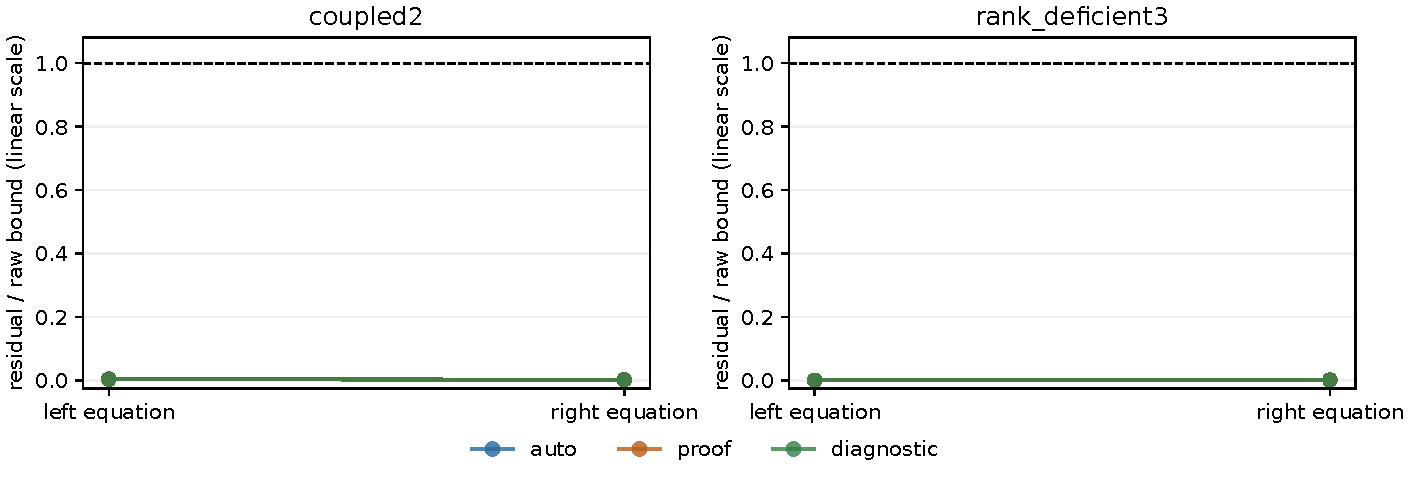
\includegraphics[width=.96\linewidth]{figures/residuals.pdf}
\caption{Raw-array residuals divided by $256n\epsilon\norm{B_2}$ or
$256n\epsilon\norm{B_3}$, respectively. Smaller is better; the horizontal
bound is 1. Zero observations are drawn at zero on a linear axis. The plot
shows the fixed cases only; the three profiles coincide here. It does
not establish a general error theorem.}
\label{fig:residuals}
\end{figure}}{}

The source distribution supplies tests, a fresh-install procedure, effective
settings, fixed-case benchmark scripts and compact results. Build, solve and
optional exact verification times are recorded separately. The accompanying curated source distribution contains the installation,
test and reproduction instructions together with these fixed-case data.
Its repository record identifies the immutable release revision.

\paragraph{AI assistance.}
The argument reconstruction, implementation, API, tests, benchmarks and writing
were produced with AI-agent assistance under the author's direction. AI review
and finite tests do not imply independent human review, formal proof
certification or acceptance by a problem repository.

\begin{thebibliography}{9}
\bibitem{open} N.~Amsel et al., \emph{Linear Systems and Eigenvalue Problems:
Open Questions from a Simons Workshop}, arXiv:2602.05394, version 3, 2026,
Section 3.4, Problem 3.8. \url{https://arxiv.org/abs/2602.05394}.
\bibitem{GL} B.~Gro{\ss}er and B.~Lang, An $O(n^2)$ algorithm for the
bidiagonal SVD, \emph{Linear Algebra Appl.} \textbf{358} (2003), 45--70.
\href{https://doi.org/10.1016/S0024-3795(01)00398-6}{doi:10.1016/S0024-3795(01)00398-6}.
\bibitem{MDV} O.~Marques, J.~Demmel and P.~B.~Vasconcelos,
\emph{Bidiagonal SVD Computation via an Associated Tridiagonal Eigenproblem},
LAPACK Working Note 295, ICL-UT-18-02, 2018.
\url{https://icl.utk.edu/files/publications/2018/icl-utk-1040-2018.pdf}.
\bibitem{Axler} S.~Axler, \emph{Linear Algebra Done Right}, 4th ed.,
Springer, 2024, Theorem 7.29. \url{https://linear.axler.net/LADR4e.pdf}.
\bibitem{Cauchy} A.~V.~Sutherland, \emph{18.785 Number theory I, Lecture \#16: Riemann's zeta function and the prime number theorem}, MIT, 2025,
Theorem 16.26. \url{https://math.mit.edu/classes/18.785/2025/LectureNotes16.pdf}.
\bibitem{Boost} Boost Multiprecision, \emph{cpp\_bin\_float}, Boost 1.89.0
documentation. \url{https://www.boost.org/doc/libs/1_89_0/libs/multiprecision/doc/html/boost_multiprecision/tut/floats/cpp_bin_float.html}.
\end{thebibliography}
\end{document}
